% Options for packages loaded elsewhere
\PassOptionsToPackage{unicode}{hyperref}
\PassOptionsToPackage{hyphens}{url}
\PassOptionsToPackage{dvipsnames,svgnames,x11names}{xcolor}
%
\documentclass[
  letterpaper,
  DIV=11,
  numbers=noendperiod]{scrartcl}

\usepackage{amsmath,amssymb}
\usepackage{lmodern}
\usepackage{iftex}
\ifPDFTeX
  \usepackage[T1]{fontenc}
  \usepackage[utf8]{inputenc}
  \usepackage{textcomp} % provide euro and other symbols
\else % if luatex or xetex
  \usepackage{unicode-math}
  \defaultfontfeatures{Scale=MatchLowercase}
  \defaultfontfeatures[\rmfamily]{Ligatures=TeX,Scale=1}
  \setmainfont[]{Times New Roman}
\fi
% Use upquote if available, for straight quotes in verbatim environments
\IfFileExists{upquote.sty}{\usepackage{upquote}}{}
\IfFileExists{microtype.sty}{% use microtype if available
  \usepackage[]{microtype}
  \UseMicrotypeSet[protrusion]{basicmath} % disable protrusion for tt fonts
}{}
\makeatletter
\@ifundefined{KOMAClassName}{% if non-KOMA class
  \IfFileExists{parskip.sty}{%
    \usepackage{parskip}
  }{% else
    \setlength{\parindent}{0pt}
    \setlength{\parskip}{6pt plus 2pt minus 1pt}}
}{% if KOMA class
  \KOMAoptions{parskip=half}}
\makeatother
\usepackage{xcolor}
\setlength{\emergencystretch}{3em} % prevent overfull lines
\setcounter{secnumdepth}{-\maxdimen} % remove section numbering
% Make \paragraph and \subparagraph free-standing
\ifx\paragraph\undefined\else
  \let\oldparagraph\paragraph
  \renewcommand{\paragraph}[1]{\oldparagraph{#1}\mbox{}}
\fi
\ifx\subparagraph\undefined\else
  \let\oldsubparagraph\subparagraph
  \renewcommand{\subparagraph}[1]{\oldsubparagraph{#1}\mbox{}}
\fi


\providecommand{\tightlist}{%
  \setlength{\itemsep}{0pt}\setlength{\parskip}{0pt}}\usepackage{longtable,booktabs,array}
\usepackage{calc} % for calculating minipage widths
% Correct order of tables after \paragraph or \subparagraph
\usepackage{etoolbox}
\makeatletter
\patchcmd\longtable{\par}{\if@noskipsec\mbox{}\fi\par}{}{}
\makeatother
% Allow footnotes in longtable head/foot
\IfFileExists{footnotehyper.sty}{\usepackage{footnotehyper}}{\usepackage{footnote}}
\makesavenoteenv{longtable}
\usepackage{graphicx}
\makeatletter
\def\maxwidth{\ifdim\Gin@nat@width>\linewidth\linewidth\else\Gin@nat@width\fi}
\def\maxheight{\ifdim\Gin@nat@height>\textheight\textheight\else\Gin@nat@height\fi}
\makeatother
% Scale images if necessary, so that they will not overflow the page
% margins by default, and it is still possible to overwrite the defaults
% using explicit options in \includegraphics[width, height, ...]{}
\setkeys{Gin}{width=\maxwidth,height=\maxheight,keepaspectratio}
% Set default figure placement to htbp
\makeatletter
\def\fps@figure{htbp}
\makeatother
\newlength{\cslhangindent}
\setlength{\cslhangindent}{1.5em}
\newlength{\csllabelwidth}
\setlength{\csllabelwidth}{3em}
\newlength{\cslentryspacingunit} % times entry-spacing
\setlength{\cslentryspacingunit}{\parskip}
\newenvironment{CSLReferences}[2] % #1 hanging-ident, #2 entry spacing
 {% don't indent paragraphs
  \setlength{\parindent}{0pt}
  % turn on hanging indent if param 1 is 1
  \ifodd #1
  \let\oldpar\par
  \def\par{\hangindent=\cslhangindent\oldpar}
  \fi
  % set entry spacing
  \setlength{\parskip}{#2\cslentryspacingunit}
 }%
 {}
\usepackage{calc}
\newcommand{\CSLBlock}[1]{#1\hfill\break}
\newcommand{\CSLLeftMargin}[1]{\parbox[t]{\csllabelwidth}{#1}}
\newcommand{\CSLRightInline}[1]{\parbox[t]{\linewidth - \csllabelwidth}{#1}\break}
\newcommand{\CSLIndent}[1]{\hspace{\cslhangindent}#1}

\usepackage{booktabs}
\usepackage{longtable}
\usepackage{array}
\usepackage{multirow}
\usepackage{wrapfig}
\usepackage{float}
\usepackage{colortbl}
\usepackage{pdflscape}
\usepackage{tabu}
\usepackage{threeparttable}
\usepackage{threeparttablex}
\usepackage[normalem]{ulem}
\usepackage{makecell}
\usepackage{xcolor}
\KOMAoption{captions}{tableheading}
\makeatletter
\makeatother
\makeatletter
\makeatother
\makeatletter
\@ifpackageloaded{caption}{}{\usepackage{caption}}
\AtBeginDocument{%
\ifdefined\contentsname
  \renewcommand*\contentsname{Table of contents}
\else
  \newcommand\contentsname{Table of contents}
\fi
\ifdefined\listfigurename
  \renewcommand*\listfigurename{List of Figures}
\else
  \newcommand\listfigurename{List of Figures}
\fi
\ifdefined\listtablename
  \renewcommand*\listtablename{List of Tables}
\else
  \newcommand\listtablename{List of Tables}
\fi
\ifdefined\figurename
  \renewcommand*\figurename{Figure}
\else
  \newcommand\figurename{Figure}
\fi
\ifdefined\tablename
  \renewcommand*\tablename{Table}
\else
  \newcommand\tablename{Table}
\fi
}
\@ifpackageloaded{float}{}{\usepackage{float}}
\floatstyle{ruled}
\@ifundefined{c@chapter}{\newfloat{codelisting}{h}{lop}}{\newfloat{codelisting}{h}{lop}[chapter]}
\floatname{codelisting}{Listing}
\newcommand*\listoflistings{\listof{codelisting}{List of Listings}}
\makeatother
\makeatletter
\@ifpackageloaded{caption}{}{\usepackage{caption}}
\@ifpackageloaded{subcaption}{}{\usepackage{subcaption}}
\makeatother
\makeatletter
\@ifpackageloaded{tcolorbox}{}{\usepackage[many]{tcolorbox}}
\makeatother
\makeatletter
\@ifundefined{shadecolor}{\definecolor{shadecolor}{rgb}{.97, .97, .97}}
\makeatother
\makeatletter
\makeatother
\ifLuaTeX
  \usepackage{selnolig}  % disable illegal ligatures
\fi
\IfFileExists{bookmark.sty}{\usepackage{bookmark}}{\usepackage{hyperref}}
\IfFileExists{xurl.sty}{\usepackage{xurl}}{} % add URL line breaks if available
\urlstyle{same} % disable monospaced font for URLs
\hypersetup{
  pdfauthor={Equipo EDUMER},
  colorlinks=true,
  linkcolor={blue},
  filecolor={Maroon},
  citecolor={Blue},
  urlcolor={Blue},
  pdfcreator={LaTeX via pandoc}}

\author{Equipo EDUMER}
\date{}

\begin{document}
\ifdefined\Shaded\renewenvironment{Shaded}{\begin{tcolorbox}[frame hidden, breakable, enhanced, borderline west={3pt}{0pt}{shadecolor}, interior hidden, sharp corners, boxrule=0pt]}{\end{tcolorbox}}\fi

\hypertarget{the-socialization-of-meritocracy-and-market-justice-preferences-at-school}{%
\section{The socialization of meritocracy and market justice preferences
at
school}\label{the-socialization-of-meritocracy-and-market-justice-preferences-at-school}}

\hypertarget{introduction}{%
\subsection{Introduction}\label{introduction}}

Since its origins, educational institutions have been related to the
idea of social mobility and access to better opportunities. Therefore,
the consistent evidence of the high level of social reproduction at the
school level represents a threat to the promise of education and a
meritocratic system
(\protect\hyperlink{ref-bourdieu_reproduction_1990}{Bourdieu \&
Passeron, 1990}). A large part of the research in this field at an
international level has addressed the extent to which the social origin
of students affects their academic results and their life opportunities
(\protect\hyperlink{ref-vonhippel_test_2019}{Von Hippel \& Hamrock,
2019}), confirming that schools have severe difficulties in closing the
gaps of origin. Besides this socioeconomic perspective on school
opportunities, recent research has addressed to what extent inequalities
in the school context are also influencing students' perceptions,
beliefs, and attitudes: Are social inequalities perceived at the school
context? Are they rejected by the students, particularly those who are
worst-off in socioeconomic terms? Or, Is there evidence at the school
level that social inequalities are tolerated and even justified?
(\protect\hyperlink{ref-batruch_belief_2022}{Batruch et al., 2022};
\protect\hyperlink{ref-wiederkehr_belief_2015}{Wiederkehr et al.,
2015}).

In the present paper, we deal with the justification of social
inequalities by eighth-grade students in Chile, a country characterized
by a highly stratified educational system. In particular, we focus on
market justice preferences
(\protect\hyperlink{ref-lane_market_1986}{Lane, 1986}), which refer to
the preferences for distributing public goods (as health and education)
based on criteria such as competition and payment capacity. Although
from a rational point of view it could be expected an opposition to
market justice by the underprivileged majority, we argue that in a
social environment characterized by a promotion of meritocratic ideals -
as the school system - would lead to the opposite: a larger market
justice preferences.

Given that the school environment has an important focus on performance,
achievement and acknowledgment, meritocracy has been one of the
principal concepts used for understanding and even for justifying
performance differences among students. Meritocracy is a distributive
system based on the belief that people should be rewarded and promoted
based on their abilities, knowledge, and achievements
(\protect\hyperlink{ref-young_rise_1958}{Young, 1958}). It is often seen
as a way to create equal opportunities and fairness, as individuals can
rise to positions of power and influence based on their own merit rather
than their background or connections. However, some argue that
meritocracy can actually lead to tolerating or even justifying social
inequalities, as it can create a hierarchy where those who already have
resources and advantages are more likely to succeed. In this regard, a
great deal of academic research about meritocracy delves into the
assessment of to what extent rewards and privileges in society are
related to merit, emphasizing the so-called unfulfillable promise of
meritocracy (\protect\hyperlink{ref-mijs_stratified_2016}{Mijs, 2016}).
Complementing this agenda, a second and emerging research area deals
with subjective aspects of meritocracy, such as perceptions and beliefs.

{[}definición de market justice, welfare marketization, (Lindh){]}

{[}contexto Chileno market justice, dar cifras/porcentajes de
privatización de salud, educación y pensiones; asociar al tema de la
calidad (lo público es peor){]}

The perception of meritocracy refers to how individuals view and
understand the concept of meritocracy in their own society
(\protect\hyperlink{ref-castillo_meritocracia_2019}{Castillo et al.,
2019}; \protect\hyperlink{ref-duru-bellat_who_2012}{Duru-Bellat \&
Tenret, 2012}). This perception can vary greatly depending on individual
experiences, social, economic, and cultural background. Some people may
see meritocracy as a fair and just system that allows anyone to succeed
based on their abilities and hard work. In contrast, others may view it
as a myth or a cover for existing power dynamics and inequality, serving
to maintain and even reinforce inequality
(\protect\hyperlink{ref-lampert_meritocratic_2013}{Lampert, 2013};
\protect\hyperlink{ref-mijs_paradox_2021}{Mijs, 2021}). Based in this
last perspective, we argue that individuals with a higher perception of
meritocracy will show a larger justification of social inequalities, as
individual achievement would be seen as rewarded and social policies as
less necessary (\protect\hyperlink{ref-batruch_belief_2022}{Batruch et
al., 2022}).

Most of the research that has related meritocratic beliefs to inequality
justification so far has only considered adults, leaving aside the study
of how beliefs in this field develop at student age as well as the
impact of the school context and the family as the main socialization
agencies. Regarding schools, the way in which they deal with unequal
conditions of origin has been linked to the \emph{hidden curriculum}
(\protect\hyperlink{ref-chafel_schooling_1997}{Chafel, 1997}), whereby
students learn about distributive norms in society and mechanisms of
justification of social differences. Based on recent studies that relate
school meritocracy to the justification of economic inequalities in the
adult population (\protect\hyperlink{ref-batruch_belief_2022}{Batruch et
al., 2022}; \protect\hyperlink{ref-wiederkehr_belief_2015}{Wiederkehr et
al., 2015}), the central hypothesis guiding this research is that
school-age students with a higher perception of meritocracy - both at
school and at the societal level - will show a larger justification of
social inequalities, as individual achievement would be seen as
appropriately rewarded and social mechanisms for correcting inequalities
as less necessary (\protect\hyperlink{ref-batruch_belief_2022}{Batruch
et al., 2022}).

\textasciitilde{}

{[}introducir distinción sobre percepción de meritocracia a nivel
escolar y a nivel de la sociedad{]}

{[}resaltar 3 focos de innovación: market justice preferences at school
level, relación con meritocracia, y esquema de meritocracia en la
escuela y en la sociedad{]}

The present paper deals with the association between the perception of
meritocracy and the justification of social inequalities, with two main
focuses. Firstly, it assesses the justification of social inequalities
in social policy domains, such as health, pensions, and education. We
argue that individuals who perceive more meritocracy would be more
willing to justify better services in these domains for those with
higher incomes. Secondly, we focus on the student-age population as we
point out that it is possible to track down the origin of meritocratic
beliefs (and their consequences) to early socialization processes. To
this regard, we take into account the family and the school as two main
socialization agencies that play a significant role in the socialization
of cultural beliefs by transmitting cultural norms, values, and
expectations to young people.

\hypertarget{justification-of-inequality}{%
\subsection{Justification of
inequality}\label{justification-of-inequality}}

Research on social stratification beliefs, which explore individual
perceptions of who deserves what and why
(\protect\hyperlink{ref-kluegel_beliefs_1987}{Kluegel \& Smith, 1987}),
highlights that people's explanations and justifications of social
inequality are closely tied to their judgments of deservingness. The
influence of ideologies
(\protect\hyperlink{ref-wegener_dominant_1995}{Wegener \& Liebig, 1995})
and cultural schemas (\protect\hyperlink{ref-homan_being_2017}{Homan et
al., 2017}) is pivotal in shaping these explanations by offering
symbolic representations that frame societal structures and
expectations. While significant attention has been paid to wage
inequality, income distribution, and payment differentials in the
literature {[}Castillo
(\protect\hyperlink{ref-castillo_legitimacy_2011}{2011}); Evans et al.,
2010; Jasso (\protect\hyperlink{ref-jasso_how_1999}{1999}) ; Shariff et
al. (\protect\hyperlink{ref-shariff_income_2016}{2016}){]}, there has
been less examination of public beliefs about which life domains should
be governed by market relations and even less about children's
acceptance or rejection of these market principles. This oversight is
notable given the extensive encroachment of market logic into public
goods, welfare policy, and social services over the past five decades
(\protect\hyperlink{ref-centeno_arc_2012}{Centeno \& Cohen, 2012};
\protect\hyperlink{ref-harvey_breve_2015}{Harvey, 2015}), affecting
areas such as pensions, health services, and education. The
justification of social inequality based on marketype criteria has been
conceptualized as the individuals' adherence to one specific justice
evaluation, the market justice, that is, affording legitimacy to the
allocation of goods and services based on prices and individuals'
ability to pay (\protect\hyperlink{ref-boltanski_new_2005}{Boltanski \&
Chiapello, 2005}; \protect\hyperlink{ref-lane_market_1986}{Lane, 1986};
\protect\hyperlink{ref-streeck_citizens_2012}{Streeck, 2012}).

Robert E. Lane proposed the underpinnings of market justice, which he
differentiated from political justice. For him, ``it is the genius of
the market to stimulate wants without at the same time stimulating a
sense of deserving more than one gets'' {[}-Lane
(\protect\hyperlink{ref-lane_market_1986}{1986}); p.~384{]}. Following
the theory of relative deprivation --a social phenomenon arising when
individuals cannot afford what most others in their environment can
(Merton 1950)-- Lane notes that, in market settings, social comparisons
are more likely to motivate increased effort rather than feelings of
acute injustice because individuals attribute outcomes to their actions.
Although empirical research has shown that, contrary to Lane's
observation, relative deprivation, even in market settings, produces
feelings of dissatisfaction, anger, and resentment that might motivate
forms of collective action such as protests and revolt
(\protect\hyperlink{ref-greitemeyer_subjective_2016}{Greitemeyer \&
Sagioglou, 2016}; \protect\hyperlink{ref-mishra_subjective_2015}{Mishra
\& Carleton, 2015};
\protect\hyperlink{ref-power_deprivationprotest_2018}{Séamus A. Power,
2018}; \protect\hyperlink{ref-power_relative_2020}{Séamus A. Power et
al., 2020}; \protect\hyperlink{ref-smith_relative_2012}{Smith et al.,
2012}), the conceptualization of market justice has been since then
closely coupled to the merit principle for allocating outcomes: the
claim that the unequal levels of well-being individuals enjoy ought to
be, to some extent, a function of their talents and efforts, regardless
of their needs or membership, the two latter being the realm of
political justice and its closely coupled principles of need
--allocating outcomes to those who require them most-- and equality
--allocating the same outcome to everyone--, which have been at the
center of welfarism (see Wilson 2003). The underlying notion of market
justice also resonates in its application to welfare regimes, providing
a framework for understanding the varied global approaches to managing
social services.

The management of social services manifests in varying approaches across
nations, with substantial differences in funding and delivery methods
(\protect\hyperlink{ref-jensen_worlds_2008}{Jensen, 2008};
\protect\hyperlink{ref-stoy_worlds_2014}{Stoy, 2014}). Nordic countries,
for example, predominantly employ public agencies to produce and provide
social services, funding these through collective taxation and offering
them in kind to the majority of citizens. This system prioritizes
political justice, placing it above market mechanisms in accessing
services. In contrast, other countries rely more heavily on for-profit
entities and private funding, where service distribution depends mainly
on individual financial capacity of paying user fees, highlighting the
influence of market justice in service allocation. The trend toward
marketization of welfare services has been growing since the 1980s
(\protect\hyperlink{ref-salamon_marketization_1993}{Salamon, 1993}), and
this shift is increasingly evident even in countries where market
solutions have traditionally had a minor role in social policy
(\protect\hyperlink{ref-sivesind_changing_2017}{Sivesind, 2017}).

The question arises whether adults and children justify unequal access
to welfare services based on market justice principles. Influenced by
theories of policy feedback, which suggest that social welfare policies
can reinforce (positive feedback) or undermine (negative feedback)
previous policy trajectories
(\protect\hyperlink{ref-fernandez_positive_2013}{Fernandez \&
Jaime-Castillo, 2013};
\protect\hyperlink{ref-pierson_increasing_2000}{Pierson, 2000};
\protect\hyperlink{ref-weaver_paths_2010}{Weaver, 2010}), citizens'
beliefs about market justice are likely also shaped by the institutional
and social contexts they encounter. Indeed, the justification of
inequality in access to essential services like education and health,
based on one's ability to pay, shows significant variation across
countries, as demonstrated by international surveys, although they do
not usually include children in their samples. For instance, the 2019
International Social Survey Program (ISSP) provides insights into how
adults perceive inequality in accessing welfare services.
Figure~\ref{fig-issp} illustrates the variation in agreement levels
regarding whether it is just for individuals with higher incomes to
purchase better education or healthcare. Notably, in 18 of the 29
countries analyzed, there is a greater justification for market
inequality in healthcare access than in education. Nevertheless, the
general sentiment typically ranges from `somewhat unjust' to 'neither
just nor unjust, with mixed feelings.

\begin{figure}

{\centering 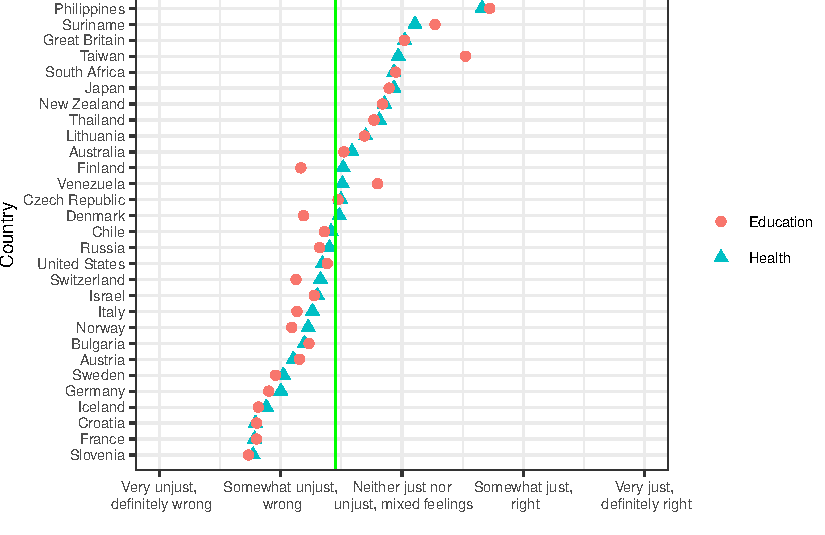
\includegraphics{paper_files/figure-pdf/fig-issp-1.pdf}

}

\caption{\label{fig-issp}Average of market justice preferences by
country}

\end{figure}

While contemporary policy developments have increasingly embraced the
marketization of social welfare in areas such as education, pensions,
and health services, questions about public acceptance of these changes
persist. Lindh (\protect\hyperlink{ref-lindh_public_2015}{2015})
analysis of ISSP 2009 data from 17 OECD countries reveals a general lack
of support for market-based distribution of social services, suggesting
widespread disapproval of market stratification of essential services.
This finding is corroborated by Soler-Martínez et al.
(\protect\hyperlink{ref-soler-martinez_concerns_2023}{2023}) research
from Latinobarómetro 2020 across 18 Latin American countries, where
concerns about health and education access predominated over income
inequality. These results indicate that reforms toward welfare
marketization are typically driven by elite political decisions rather
than grassroots demand.

Despite high-income inequality and limited social mobility in Latin
America, there is a prevalent belief that individuals are solely
responsible for their economic outcomes, a view that varies across the
region (\protect\hyperlink{ref-bucca_merit_2016}{Bucca, 2016};
\protect\hyperlink{ref-chong_mystery_2008}{Chong \& Ñopo, 2008};
\protect\hyperlink{ref-salgado_inequality_2023}{Salgado \& Castillo,
2023}; \protect\hyperlink{ref-torche_intergenerational_2014}{Torche,
2014}). The reliance on private welfare providers and widespread user
fees (\protect\hyperlink{ref-molyneux_neoliberal_2008}{Molyneux, 2008})
adds complexity to this context. Yet, research on children's
justification of market-based inequalities in accessing welfare services
remains limited, especially in Latin America, highlighting a significant
gap in understanding how younger generations view market-based access to
welfare and whether these views are associated with their meritocratic
beliefs.

\hypertarget{meritocracy}{%
\subsection{Meritocracy}\label{meritocracy}}

The concept of meritocracy frequently appears nowadays when analyzing
cultural determinants of social inequalities. In general, it is
mentioned as a value associated with justice, as it would link efforts
and talents with rewards in an equitable manner. This normative sense is
quite far from its original formulation by Young
(\protect\hyperlink{ref-young_rise_1958}{1958}) in the satirical novel
``The Rise of Meritocracy'', where it ironically represented a mechanism
for reproducing the inequalities of origin. The meritocratic ideal had
remained relatively unchallenged until a series of recent publications
turned into its potential consequences for maintaining social
inequality. Perhaps one of the most recent sources in this line is
Michael Sandel's ``The Tyranny of Merit'', where he strongly questions
the implications of carrying out the principle of merit in societies
that do not guarantee equal opportunities and that generate a feeling of
scarce recognition and appreciation of those who receive lesser rewards:
``In society's eyes, and perhaps also their own, their work no longer
signified a valued contribution to the common good.''
(\protect\hyperlink{ref-sandel_tyranny_2020}{Sandel, 2020}, pp.).

Empirical research on meritocracy has increased along with the
philosophical-normative discussion on meritocracy in recent years.
Particularly from a sociological perspective, meritocracy has been used
in research on social mobility to characterize societies with low
mobility that threaten the meritocratic ideal
(\protect\hyperlink{ref-goldthorpe_myth_2003}{Goldthorpe, 2003}). More
recently, sociology and social psychology research has attended to the
subjective aspects vis-a-vis beliefs in meritocracy. The label of
beliefs in this realm covers a series of areas, such as attitudes,
perceptions, and preferences (Castillo et al), whereby most of the link
this subjective dimensions to individual socio-structural factors and
context-level determinants. For instance, some studies have analyzed how
those with greater privileges believe more in meritocracy (Reynolds \&
Chan 2014), how greater economic inequality increases meritocratic
beliefs (\protect\hyperlink{ref-mijs_paradox_2021}{Mijs, 2021}), and how
larger inequality affects meritocratic beliefs
(\protect\hyperlink{ref-morris_representing_2022}{Morris et al., 2022}).
Based on these findings, a research agenda has been reinforced on the
legitimizing role of meritocracy, in line with previous studies using
the concept of a just world (Lerner, Dalbert) and the theory of system
justification (Jost \& Major).

How do meritocratic beliefs legitimize inequalities? Empirical studies
have used experiments and surveys to address this question. For
instance, the evidence suggests that just world beliefs correlate
negatively with support for redistributive compensation systems
(\protect\hyperlink{ref-frank_performance_2015}{Frank et al., 2015}).
Conversely, individuals tend to support redistribution when they believe
that the disadvantaged lack the opportunities to succeed
(\protect\hyperlink{ref-evans_strong_2018}{Evans \& Kelley, 2018}).
Almås et al. (\protect\hyperlink{ref-almas_cutthroat_2020}{2020}) found
that in a relatively unequal society (the United States), the highly
educated accept inequality significantly more than the less educated
because they perceive inequality as justifiable owing to differences in
productivity (i.e., merit), whereas in a relatively equal society
(Norway), the less educated accept inequality more, but not
significantly more than the highly educated because meritocratic values
are less prevalent. Barr \& Miller
(\protect\hyperlink{ref-barr_effect_2020}{2020}) also addressed this
triple interaction between the level of inequality in a society, the
individual level of education, and the perceived origin of the disparity
(either by luck or effort) to determine the extent to which inequality
is accepted. They found that the interaction's mechanism varies
depending on the compared societies. Finally, García-Sánchez et al.
(\protect\hyperlink{ref-garcia-sanchez_attitudes_2020}{2020}), using
data for 41 countries from the International Social Survey Programme
(ISSP), found that the perceived size of the income gap correlated
positively with support for progressive taxation. Still, this
association was weaker among those who endorsed meritocratic and equal
opportunity beliefs. In the same line, experimental research by Durante
\& Putterman (\protect\hyperlink{ref-durante_preferences_2009}{2009})
subjects support less redistribution when the initial distribution is
determined according to task performance.

Research about meritocratic beliefs at school age is rather scarce,
leaving a wide research gap as schools are one of the primary
socialization institutions where achievement based on merit explains
success (\protect\hyperlink{ref-erivwo_meritocracy_2021}{Erivwo et al.,
2021}). Nevertheless, it is possible to find some initial works focused
on the area of distributive justice at school that are closely related
to meritocratic beliefs, as the ones by Resh and Sabbagh (quotes). Using
justice in grade obtention as a measure of distributive justice and
meritocracy (Sabbagh et al 2006), they find for instance that a larger
sense of distributive justice about grades is associated to higher
socio-economic status (\protect\hyperlink{ref-resh_sense_2010}{Resh,
2010}), have a positive effect on liberal democratic orientation and on
trust in people and in formal institutions
(\protect\hyperlink{ref-resh_sense_2014}{Resh \& Sabbagh, 2014}), and
tend to refrain from violence and to engage to a greater extent in
extra-curricular school activity and community volunteering
(\protect\hyperlink{ref-resh_sense_2017}{Resh \& Sabbagh, 2017}).

\hypertarget{childrens-judgments-of-inequality-schools-and-family-background}{%
\subsection{Children's judgments of inequality, schools, and family
background}\label{childrens-judgments-of-inequality-schools-and-family-background}}

Research indicates various socialization practices at families and
schools during childhood and adolescence that impact dispositional and
behavioral tendencies concerning justifications of inequality in adult
life. The differences in economic understanding across age groups are
consistent with research on cognitive development
(\protect\hyperlink{ref-choudhury_social_2006}{Choudhury et al., 2006}).
Adolescents with mature socio-cognitive abilities tend to express
stronger preferences for fairness than infants and children
(\protect\hyperlink{ref-wynn_not_2018}{Wynn et al., 2018}). As children
grow older, they become more likely to behave fairly, with their
early-emerging strict egalitarianism being replaced by an increasing
endorsement of fairness principles and engagement in collaborative
activities (\protect\hyperlink{ref-huppert_development_2019}{Huppert et
al., 2019};
\protect\hyperlink{ref-mcauliffe_developmental_2017}{McAuliffe et al.,
2017}). In these activities, their fairness views consider individual
contributions, merits, and circumstances
(\protect\hyperlink{ref-almas_fairness_2010}{Almås et al., 2010};
\protect\hyperlink{ref-huppert_development_2019}{Huppert et al., 2019};
\protect\hyperlink{ref-sigelman_development_1991}{Sigelman \& Waitzman,
1991}). Engelmann \& Tomasello
(\protect\hyperlink{ref-engelmann_children_2019}{2019}) claim that
children's sense of fairness emerges at three years old, and we can
observe it in collaborative activities, where they accept inequality if
the procedure gives everyone an equal chance. Therefore, children at
this age respond to unequal distributions based on interpersonal
concerns, as they already demand equal respect. In any case, between 3
and 8 years of age, inequitable and anti-meritorious allocations are
evaluated more negatively, but equitable and meritorious allocations are
not evaluated more positively
(\protect\hyperlink{ref-elenbaas_unfairness_2019}{Elenbaas, 2019}).

Some research shows that the social environment in which children
develop, such as family and school, is associated with their prosocial
behaviors by playing an essential role in the transmission of equity
norms (\protect\hyperlink{ref-kosse_prosociality_2020}{Kosse \& Tincani,
2020}; \protect\hyperlink{ref-schunk_fairness_2023}{Schunk \& Zipperle,
2023}). In fact, schools contribute to institutionalizing and
reproducing inequality by promoting values, norms, practices, and
languages familiar to higher-class families because the dominant group's
culture shapes educational institutions
(\protect\hyperlink{ref-bourdieu_reproduction_1990}{Bourdieu \&
Passeron, 1990}). Middle- and upper-class students are better equipped
to face academic challenges and are more familiar with academic
expectations (\protect\hyperlink{ref-mikus_children_2020}{Mikus et al.,
2020}). Such familiarity represents cultural capital in educational
contexts because higher-status students come to school ready to meet
these expectations and reap the benefits
(\protect\hyperlink{ref-jack_no_2016}{Jack, 2016};
\protect\hyperlink{ref-khan_privilege_2011}{Khan, 2011}). Conversely,
lower-status children lacking cultural capital must catch up while
experiencing inequitable comparisons
(\protect\hyperlink{ref-goudeau_hidden_2017}{Goudeau \& Croizet, 2017}).
Additionally, academic achievement is treated as the outcome of
dispositional factors (e.g., pupils' efforts and talents or lack of
them) rather than the result of differential access to critical
resources. Due to the meritocratic frame schools encourage, both low-
and high-status individuals believe that students' success or failure is
not due to their family background but rather to differences in efforts
and talents (\protect\hyperlink{ref-darnon_where_2018}{Darnon et al.,
2018}). In this sense, we believe that the perception of meritocracy can
influence students' judgments about market justice preferences.
Furthermore, we believe there is a difference between students'
perceptions of meritocracy based on their own experience in school and
what they perceive in society at large. Consistently, our first two
hypotheses are:

H1a: Students who perceive that there is more meritocracy at school will
show larger market justice preferences

H1b: Students who perceive that there is more meritocracy in society
will show larger market justice preferences

Family background and family socialization practices also contribute to
children's and adolescent's market justice preferences. For example,
Almås et al. (\protect\hyperlink{ref-almas_fairness_2017}{2017}) found
that adolescents from low-socioeconomic-status families are likelier to
have an egalitarian fairness view and consider an equal distribution as
fair in a situation with unequal merits. The authors speculate that
differences in socialization practices across status groups might bring
about, to a great extent, the fairness views of children and adolescents
because social status seems to interact with these evaluations (e.g.,
\protect\hyperlink{ref-hvidberg_social_2023}{Hvidberg et al., 2023}).

The classic work of Kohn showed that middle-class parents value the
expression of internal states and emotions, such as self-control,
curiosity, happiness, and consideration, while working-class parents
promote deference, obedience, and conformity to authority
(\protect\hyperlink{ref-kohn_social_1963}{Kohn, 1963};
\protect\hyperlink{ref-kohn_class_1969}{Kohn \& Schooler, 1969}).
Although parents from all social backgrounds encourage individualism in
their children, this shared norm translates into different forms in high
and low social classes (1999). Acemoglu
(\protect\hyperlink{ref-acemoglu_obedience_2021}{2021}) claimed that the
values families impart to their children interact with social mobility.
Because obedience is a valuable characteristic for employers, in
low-wage and social mobility environments, low-income families impart
values of obedience to their children to prevent disadvantaging them in
labor markets. On the one hand, children from privileged families are
socialized to adopt a clear conception of individualism that highlights
their internal states, independence, and idiosyncrasies. In contrast,
children from disadvantaged families are socialized to support a more
balanced view of individualism that considers personal characteristics
as resources to overcome collective impediments on the path to upward
mobility
(\protect\hyperlink{ref-iacoviello_collectivism_2019}{Iacoviello \&
Lorenzi-Cioldi, 2019}). In this way, we believe that there are
differences in the socialization of values according to socioeconomic
differences that could influence market justice preferences and,
therefore, we propose the following hypothesis:

H2: Students from families of higher social status will show larger
market justice preferences.

Recent empirical research has demonstrated that the institutional design
of schools, coupled with the meritocratic ideology it fosters,
significantly influences children's and adolescents' views on inequality
and deservingness. For example, Jonsson \& Beach
(\protect\hyperlink{ref-jonsson_institutional_2015}{2015}) study
revealed that higher-status adolescents in Sweden tend to perpetuate
social class stereotypes while describing the vocational and academic
tracks. Academic track students are depicted as wealthy, intelligent,
ambitious, and diligent, while vocational track students are
characterized as poor, unambitious, unintelligent, and lackadaisical.
These stereotypes help individuals maintain a sense of superiority over
others and legitimize the prevailing social hierarchies and economic
disparities (\protect\hyperlink{ref-jost_attitudinal_2000}{Jost \&
Burgess, 2000})

H3: Students from schools of higher social status will show larger
market justice preferences.

H4: Students from schools with higher average levels of academic
achievement will show larger market justice preferences.

{[}interacciones{]}

H5: The perception of meritocracy in school and society will moderate
the effect of family social status on market justice preferences.

H6: The perception of meritocracy in school and society will moderate
the effect of school status on market justice preferences.

H7: The perception of meritocracy in school and society will moderate
the effect of school academic achievement on market justice preferences.

\hypertarget{summary-of-hypotheses}{%
\subsubsection{Summary of hypotheses}\label{summary-of-hypotheses}}

\begin{figure}

{\centering 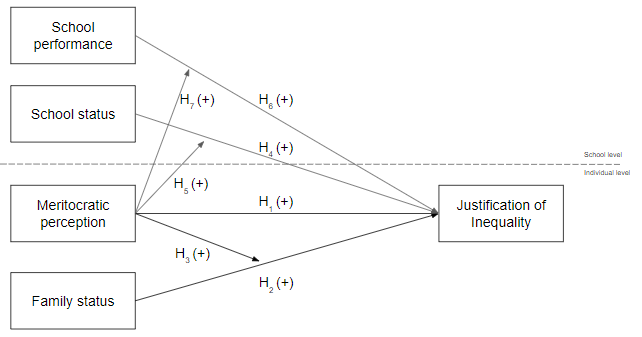
\includegraphics[width=6.25in,height=\textheight]{input/img/hypotheses.png}

}

\caption{\label{fig-hypotheses}Summary of hypotheses}

\end{figure}

\hypertarget{methods}{%
\subsection{Methods}\label{methods}}

\hypertarget{data}{%
\subsubsection{Data}\label{data}}

The main data source corresponds to the First Study of Civic Education
in Chile, conducted by the Agency for Quality Education of the Ministry
of Education in 2017. This database is based on the administration of a
civic knowledge test to students and questionnaires to various members
of the educational community. The target population consists of
8th-grade students in 242 schools across the country. Initially, the
database comprises 8,589 student observations and 6,770 parent
observations. However, considering the survey's unit of analysis and to
ensure higher data quality, 171 student cases and 79 parent cases
exhibiting repetitive and careless response patterns were removed
(Gottfried et al., 2022). Additionally, data from the System for
Measuring the Quality of Education (SIMCE) conducted by the Ministry of
Education for the year 2017 are employed, providing school-level
information such as administrative dependence, socioeconomic
classification, and results obtained in standardized mathematics and
language tests. After variable processing and removal of missing cases,
the final database for this study includes a two-level stratified
sample, composed of 5,047 students and parents (level 1) nested within
231 schools (level 2).

\hypertarget{variables}{%
\subsubsection{Variables}\label{variables}}

\textbf{\emph{Individual level}}

\textbf{Justification of Inequality}: The dependent variable in this
study is the justification of social inequality in specific policy
domains, namely health, education, and pensions. This construct is
measured through three variables addressing the degree of justification
regarding whether access to social services in these domains should be
income conditional. Justification of inequality in health is measured by
the item ``Is it fair in Chile that people with higher incomes can
access better healthcare than those with lower incomes,'' while in
education, it is measured using the statement ``Is it fair in Chile that
people who can afford it have better education for their children.'' In
the case of pensions, it is measured through the item ``Is it fair in
Chile that people with higher incomes can have better pensions than
those with lower incomes.'' In all cases, respondents declare their
preferences on a Likert scale ranging from ``completely disagree'' (1)
to ``completely agree'' (4). Additionally, we include a summarized
indicator of preferences for market justice (REF), measured by an
average index across these items (α = 0.86), with values ranging from 1
to 4, where higher values represent greater preferences for market
justice (see Table~\ref{tbl-desc-dependientes}).

\hypertarget{tbl-desc-dependientes}{}
\begin{longtable}[]{@{}
  >{\raggedright\arraybackslash}p{(\columnwidth - 6\tabcolsep) * \real{0.4286}}
  >{\raggedright\arraybackslash}p{(\columnwidth - 6\tabcolsep) * \real{0.2551}}
  >{\raggedright\arraybackslash}p{(\columnwidth - 6\tabcolsep) * \real{0.2143}}
  >{\raggedright\arraybackslash}p{(\columnwidth - 6\tabcolsep) * \real{0.1020}}@{}}
\caption{\label{tbl-desc-dependientes}Dependent
variables}\tabularnewline
\toprule()
\begin{minipage}[b]{\linewidth}\raggedright
Label
\end{minipage} & \begin{minipage}[b]{\linewidth}\raggedright
Stats / Values
\end{minipage} & \begin{minipage}[b]{\linewidth}\raggedright
Freqs (\% of Valid)
\end{minipage} & \begin{minipage}[b]{\linewidth}\raggedright
Valid
\end{minipage} \\
\midrule()
\endfirsthead
\toprule()
\begin{minipage}[b]{\linewidth}\raggedright
Label
\end{minipage} & \begin{minipage}[b]{\linewidth}\raggedright
Stats / Values
\end{minipage} & \begin{minipage}[b]{\linewidth}\raggedright
Freqs (\% of Valid)
\end{minipage} & \begin{minipage}[b]{\linewidth}\raggedright
Valid
\end{minipage} \\
\midrule()
\endhead
It is just that in Chile people with higher incomes can have better
pensions than people with low incomes &
\begin{minipage}[t]{\linewidth}\raggedright
1. Strongly disagree\\
2. Disagree\\
3. Agree\\
4. Strongly agree\strut
\end{minipage} & \begin{minipage}[t]{\linewidth}\raggedright
1837 (30.6\%)\\
1945 (32.4\%)\\
1622 (27.0\%)\\
608 (10.1\%)\strut
\end{minipage} & \begin{minipage}[t]{\linewidth}\raggedright
6012\\
(95.9\%)\strut
\end{minipage} \\
It is just that in Chile people who can pay have a better education for
their children & \begin{minipage}[t]{\linewidth}\raggedright
1. Strongly disagree\\
2. Disagree\\
3. Agree\\
4. Strongly agree\strut
\end{minipage} & \begin{minipage}[t]{\linewidth}\raggedright
1766 (29.7\%)\\
1732 (29.1\%)\\
1704 (28.6\%)\\
750 (12.6\%)\strut
\end{minipage} & \begin{minipage}[t]{\linewidth}\raggedright
5952\\
(94.9\%)\strut
\end{minipage} \\
It is just that in Chile people with higher incomes can access better
health services than people with low incomes &
\begin{minipage}[t]{\linewidth}\raggedright
1. Strongly disagree\\
2. Disagree\\
3. Agree\\
4. Strongly agree\strut
\end{minipage} & \begin{minipage}[t]{\linewidth}\raggedright
2254 (38.0\%)\\
1685 (28.4\%)\\
1401 (23.6\%)\\
593 (10.0\%)\strut
\end{minipage} & \begin{minipage}[t]{\linewidth}\raggedright
5933\\
(94.6\%)\strut
\end{minipage} \\
Market Justice Preferences & \begin{minipage}[t]{\linewidth}\raggedright
Mean (sd) : 2.2 (0.9)\\
min \textless{} med \textless{} max:\\
1 \textless{} 2 \textless{} 4\\
IQR (CV) : 1.7 (0.4)\strut
\end{minipage} & 13 distinct values &
\begin{minipage}[t]{\linewidth}\raggedright
6077\\
(96.9\%)\strut
\end{minipage} \\
\bottomrule()
\end{longtable}

\textbf{Perception of Meritocracy}: The main independent variable refers
to the perception of meritocracy, operationalized through five items
addressing the perception of rewards based on talent and intelligence at
both the school and societal levels. At the school level, students
respond to whether ``Intelligence is important for getting good grades''
and ``Effort is important for getting good grades.'' At the societal
level, students respond to the following questions: ``In Chile, people
are rewarded for their effort,'' ``In Chile, people get what they
deserve,'' and ``In Chile, people are rewarded for their intelligence
and skills.'' Each item was answered on a four-point Likert scale
ranging from ``completely disagree'' (1) to ``completely agree'' (4).

The analysis includes several individual control variables that have
been identified as influential in recent research. These variables
encompass family socioeconomic status, assessed by the highest level of
parental education, the number of books in the household, and an index
measuring access to technologies, all aimed at mitigating compositional
effects (REFS). Table~\ref{tbl-desc-independent} shows the independent
variables used, their response categories and their frequencies.

\hypertarget{tbl-desc-independent}{}
\begin{longtable}[]{@{}
  >{\raggedright\arraybackslash}p{(\columnwidth - 6\tabcolsep) * \real{0.3925}}
  >{\raggedright\arraybackslash}p{(\columnwidth - 6\tabcolsep) * \real{0.3084}}
  >{\raggedright\arraybackslash}p{(\columnwidth - 6\tabcolsep) * \real{0.1963}}
  >{\raggedright\arraybackslash}p{(\columnwidth - 6\tabcolsep) * \real{0.1028}}@{}}
\caption{\label{tbl-desc-independent}Independent
variables}\tabularnewline
\toprule()
\begin{minipage}[b]{\linewidth}\raggedright
Label
\end{minipage} & \begin{minipage}[b]{\linewidth}\raggedright
Stats / Values
\end{minipage} & \begin{minipage}[b]{\linewidth}\raggedright
Freqs (\% of Valid)
\end{minipage} & \begin{minipage}[b]{\linewidth}\raggedright
Valid
\end{minipage} \\
\midrule()
\endfirsthead
\toprule()
\begin{minipage}[b]{\linewidth}\raggedright
Label
\end{minipage} & \begin{minipage}[b]{\linewidth}\raggedright
Stats / Values
\end{minipage} & \begin{minipage}[b]{\linewidth}\raggedright
Freqs (\% of Valid)
\end{minipage} & \begin{minipage}[b]{\linewidth}\raggedright
Valid
\end{minipage} \\
\midrule()
\endhead
Intelligence is important to get good grades &
\begin{minipage}[t]{\linewidth}\raggedright
1. Strongly disagree\\
2. Disagree\\
3. Agree\\
4. Strongly agree\strut
\end{minipage} & \begin{minipage}[t]{\linewidth}\raggedright
367 ( 6.1\%)\\
920 (15.3\%)\\
2970 (49.4\%)\\
1760 (29.3\%)\strut
\end{minipage} & \begin{minipage}[t]{\linewidth}\raggedright
6017\\
(95.9\%)\strut
\end{minipage} \\
Effort is important to get good grades &
\begin{minipage}[t]{\linewidth}\raggedright
1. Strongly disagree\\
2. Disagree\\
3. Agree\\
4. Strongly agree\strut
\end{minipage} & \begin{minipage}[t]{\linewidth}\raggedright
109 ( 1.8\%)\\
88 ( 1.5\%)\\
1427 (23.7\%)\\
4406 (73.1\%)\strut
\end{minipage} & \begin{minipage}[t]{\linewidth}\raggedright
6030\\
(96.1\%)\strut
\end{minipage} \\
In Chile, people are rewarded for their intelligence and skill &
\begin{minipage}[t]{\linewidth}\raggedright
1. Strongly disagree\\
2. Disagree\\
3. Agree\\
4. Strongly agree\strut
\end{minipage} & \begin{minipage}[t]{\linewidth}\raggedright
517 ( 9.0\%)\\
1568 (27.3\%)\\
2673 (46.6\%)\\
983 (17.1\%)\strut
\end{minipage} & \begin{minipage}[t]{\linewidth}\raggedright
5741\\
(91.5\%)\strut
\end{minipage} \\
In Chile, people are rewarded for their efforts &
\begin{minipage}[t]{\linewidth}\raggedright
1. Strongly disagree\\
2. Disagree\\
3. Agree\\
4. Strongly agree\strut
\end{minipage} & \begin{minipage}[t]{\linewidth}\raggedright
512 ( 8.7\%)\\
1733 (29.4\%)\\
2607 (44.2\%)\\
1050 (17.8\%)\strut
\end{minipage} & \begin{minipage}[t]{\linewidth}\raggedright
5902\\
(94.1\%)\strut
\end{minipage} \\
In Chile, people get what they deserve &
\begin{minipage}[t]{\linewidth}\raggedright
1. Strongly disagree\\
2. Disagree\\
3. Agree\\
4. Strongly agree\strut
\end{minipage} & \begin{minipage}[t]{\linewidth}\raggedright
604 (10.5\%)\\
1911 (33.1\%)\\
2388 (41.4\%)\\
871 (15.1\%)\strut
\end{minipage} & \begin{minipage}[t]{\linewidth}\raggedright
5774\\
(92.1\%)\strut
\end{minipage} \\
Parental educational level & \begin{minipage}[t]{\linewidth}\raggedright
1. 8th grade or less\\
2. Secondary Education\\
3. Higher tec. education\\
4. University or Postgraduat\\
5. Missing\strut
\end{minipage} & \begin{minipage}[t]{\linewidth}\raggedright
559 ( 8.9\%)\\
1698 (27.1\%)\\
960 (15.3\%)\\
1080 (17.2\%)\\
1975 (31.5\%)\strut
\end{minipage} & \begin{minipage}[t]{\linewidth}\raggedright
6272\\
(100.0\%)\strut
\end{minipage} \\
Number of books at home & \begin{minipage}[t]{\linewidth}\raggedright
1. Les than 25\\
2. More than 25\strut
\end{minipage} & \begin{minipage}[t]{\linewidth}\raggedright
3920 (63.2\%)\\
2281 (36.8\%)\strut
\end{minipage} & \begin{minipage}[t]{\linewidth}\raggedright
6201\\
(98.9\%)\strut
\end{minipage} \\
Technology access index & \begin{minipage}[t]{\linewidth}\raggedright
Mean (sd) : 7.8 (2.5)\\
min \textless{} med \textless{} max:\\
0 \textless{} 8 \textless{} 12\\
IQR (CV) : 3 (0.3)\strut
\end{minipage} & 13 distinct values &
\begin{minipage}[t]{\linewidth}\raggedright
6272\\
(100.0\%)\strut
\end{minipage} \\
\bottomrule()
\end{longtable}

\textbf{\emph{Contextual level}}

This study examines four variables at the school level. Firstly, we
assess the administrative dependence of schools, categorized as
``Public,'' ``Subsidized Private,'' or ``Private.'' Secondly, we
consider the socioeconomic classification of schools, determined by the
Ministry of Education and measured on an ordinal scale with five
categories ranging from ``low'' (1) to ``high'' (5). Thirdly, we
evaluate the performance level of schools in SIMCE standardized tests,
categorized as ``low,'' ``medium,'' or ``high.'' Lastly, we analyze the
proportion of parents with university or postgraduate education level at
each school. The items used, response categories, and their frequencies
are detailed in Table~\ref{tbl-desc-school}.

\hypertarget{tbl-desc-school}{}
\begin{longtable}[]{@{}
  >{\raggedright\arraybackslash}p{(\columnwidth - 6\tabcolsep) * \real{0.4040}}
  >{\raggedright\arraybackslash}p{(\columnwidth - 6\tabcolsep) * \real{0.2626}}
  >{\raggedright\arraybackslash}p{(\columnwidth - 6\tabcolsep) * \real{0.2222}}
  >{\raggedright\arraybackslash}p{(\columnwidth - 6\tabcolsep) * \real{0.1111}}@{}}
\caption{\label{tbl-desc-school}School context variables}\tabularnewline
\toprule()
\begin{minipage}[b]{\linewidth}\raggedright
Label
\end{minipage} & \begin{minipage}[b]{\linewidth}\raggedright
Stats / Values
\end{minipage} & \begin{minipage}[b]{\linewidth}\raggedright
Freqs (\% of Valid)
\end{minipage} & \begin{minipage}[b]{\linewidth}\raggedright
Valid
\end{minipage} \\
\midrule()
\endfirsthead
\toprule()
\begin{minipage}[b]{\linewidth}\raggedright
Label
\end{minipage} & \begin{minipage}[b]{\linewidth}\raggedright
Stats / Values
\end{minipage} & \begin{minipage}[b]{\linewidth}\raggedright
Freqs (\% of Valid)
\end{minipage} & \begin{minipage}[b]{\linewidth}\raggedright
Valid
\end{minipage} \\
\midrule()
\endhead
Proportion of parents with university level by school &
\begin{minipage}[t]{\linewidth}\raggedright
Mean (sd) : 0.2 (0.2)\\
min \textless{} med \textless{} max:\\
0 \textless{} 0.1 \textless{} 0.9\\
IQR (CV) : 0.2 (0.9)\strut
\end{minipage} & 103 distinct values &
\begin{minipage}[t]{\linewidth}\raggedright
6272\\
(100.0\%)\strut
\end{minipage} \\
SIMCE score by school & \begin{minipage}[t]{\linewidth}\raggedright
1. Low\\
2. Medium\\
3. High\strut
\end{minipage} & \begin{minipage}[t]{\linewidth}\raggedright
2091 (33.3\%)\\
2091 (33.3\%)\\
2090 (33.3\%)\strut
\end{minipage} & \begin{minipage}[t]{\linewidth}\raggedright
6272\\
(100.0\%)\strut
\end{minipage} \\
Administrative dependency of school &
\begin{minipage}[t]{\linewidth}\raggedright
1. Public\\
2. Subsidized private\\
3. Private\strut
\end{minipage} & \begin{minipage}[t]{\linewidth}\raggedright
2659 (42.4\%)\\
3169 (50.5\%)\\
444 ( 7.1\%)\strut
\end{minipage} & \begin{minipage}[t]{\linewidth}\raggedright
6272\\
(100.0\%)\strut
\end{minipage} \\
Socioeconomic level of school &
\begin{minipage}[t]{\linewidth}\raggedright
1. Low\\
2. Medium low\\
3. Medium\\
4. Medium high\\
5. High\strut
\end{minipage} & \begin{minipage}[t]{\linewidth}\raggedright
720 (11.5\%)\\
2282 (36.4\%)\\
1383 (22.1\%)\\
1309 (20.9\%)\\
578 ( 9.2\%)\strut
\end{minipage} & \begin{minipage}[t]{\linewidth}\raggedright
6272\\
(100.0\%)\strut
\end{minipage} \\
\bottomrule()
\end{longtable}

\hypertarget{methods-1}{%
\subsubsection{Methods}\label{methods-1}}

Given the hierarchical structure of the data, with students nested
within schools, model estimation is performed within a multilevel
framework. These models are appropriate for capturing both individual
and contextual effects in a single analysis, allowing for the estimation
of fixed effects between groups and random effects that vary from one
group to another (\protect\hyperlink{ref-bell_fixed_2019}{Bell et al.,
2019}; \protect\hyperlink{ref-hox_multilevel_2010}{Hox et al., 2010}).
Cumulative link mixed models were employed for the ordinal dependent
variables, while linear mixed-effects models were applied for the
average market justice preference index.

The hypotheses of this research were pre-registered in the Open Science
Framework platform of the Center for Open Science (OSF), the access to
the document is available at this
\href{https://doi.org/10.17605/OSF.IO/UFSDV}{link}. The statistical
analysis of this research was performed using the free software R
version 4.1.3.

\hypertarget{analysis}{%
\subsection{Analysis}\label{analysis}}

\hypertarget{descriptive-analysis}{%
\subsubsection{Descriptive analysis}\label{descriptive-analysis}}

\begin{figure}

{\centering 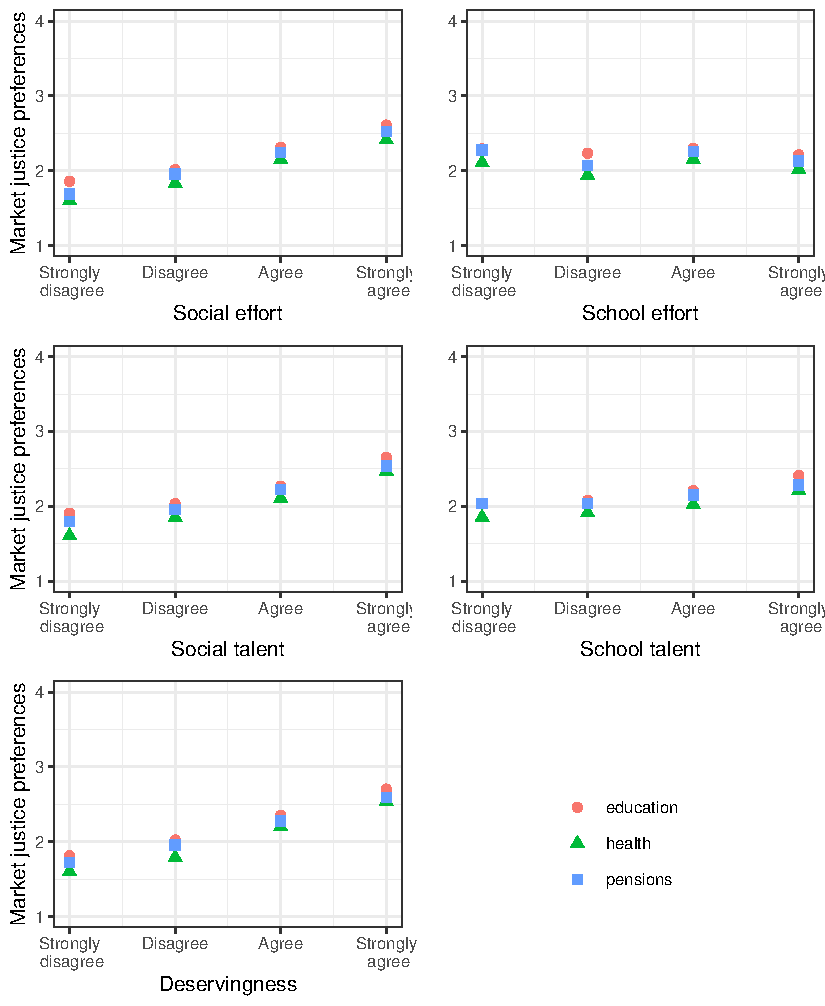
\includegraphics{paper_files/figure-pdf/fig-bivariate-1.pdf}

}

\caption{\label{fig-bivariate}Market justice preferences in education,
health and pensions by social and school meritocracy}

\end{figure}

Figure~\ref{fig-bivariate} shows a series of graphs depicting the
association between the variables of market justice preferences - in
education, health, and pensions - and the variables of meritocratic
perception at school (effort and talent) and in society (effort, talent,
and deservingness) (see conceptual diagram in
Figure~\ref{fig-hypotheses}). On the left, we observe the social
meritocracy diagrams, while on the right the school meritocracy diagrams
are shown. For the three variables of perception of meritocracy in
society the relationship is clear, since the average of market justice
preferences increases the more there is agreement that people are
rewarded for their effort, merit, and talent. This relationship needs to
be clarified in the case of the variables of perception of meritocracy
at school. To the extent that there is more agreement that the
perception of talent is essential for obtaining good grades, the average
of market justice preferences increases, but this relationship is not as
clear as with the variables of meritocracy in society. In addition, the
graph does not show a clear trend in the relationship between the
perception that effort is essential to obtain good grades and market
justice preferences.

\hypertarget{cumulative-link-mixed-models-for-the-justification-of-inequality-in-education-health-and-pensions}{%
\subsubsection{Cumulative link mixed models for the Justification of
inequality in education, health and
pensions}\label{cumulative-link-mixed-models-for-the-justification-of-inequality-in-education-health-and-pensions}}

Three Cumulative link mixed models were estimated for the ordinal
dependent variables of justice in differential access to pensions,
education, and health according to income. Figure~\ref{fig-odds} shows
the estimation of this regression model containing all the variables
used in the study for the three dependent variables separately. However,
this figure shows only the effect of meritocracy variables on society
and school as independent variables. Complete models are available in
the appendix.

\begin{figure}

{\centering 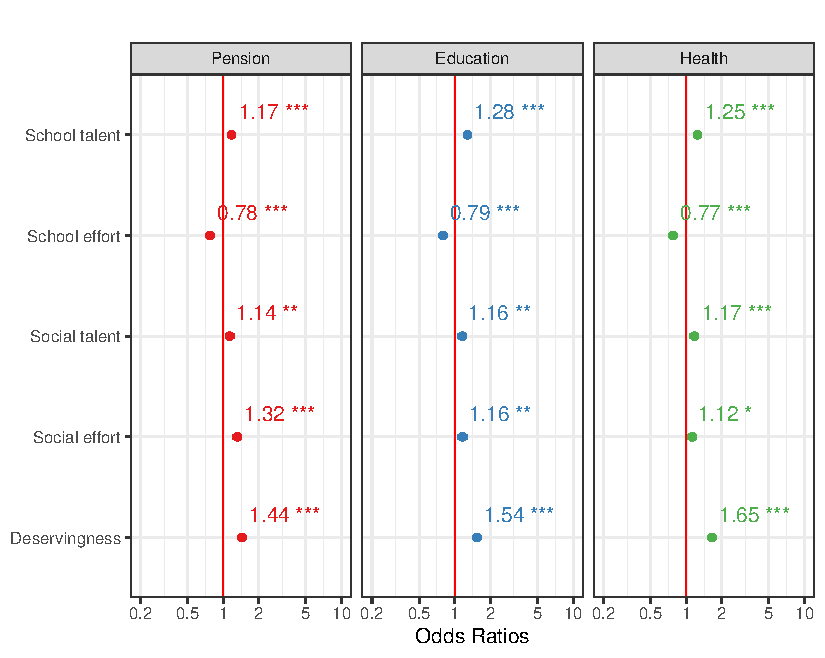
\includegraphics{paper_files/figure-pdf/fig-odds-1.pdf}

}

\caption{\label{fig-odds}Odds-ratios of justification of education,
pensions and health by social and school meritocracy}

\end{figure}

Figure~\ref{fig-odds} shows that for the three dependent variables of
justice in differential access to pensions, education, and health, the
trend is similar. In the context of school meritocracy, the effects are
mixed. As school talent increases, the justification for differentiated
access to pensions, education, and health increases; on the contrary, as
the school effort variable increases, the justification for
differentiated access to pensions, education, and health decreases,
keeping the rest of the independent variables constant. Regarding the
variables of social meritocracy, the three variables of talent, effort,
and deservingness show that as these increase, the justification for
differentiated access to pensions, education, and health also increases.

\hypertarget{multilevel-regression-models-for-market-justice-preferences}{%
\subsubsection{Multilevel regression models for market justice
preferences}\label{multilevel-regression-models-for-market-justice-preferences}}

\hypertarget{tbl-individual-reg}{}
\begin{table}
\begin{center}
\begin{tabular}{l c c}
\hline
 & Model 1 & Model 2 \\
\hline
Intercept                                    & $1.34^{***}$  & $1.37^{***}$  \\
                                             & $(0.09)$      & $(0.10)$      \\
School talent                                & $0.11^{***}$  & $0.10^{***}$  \\
                                             & $(0.01)$      & $(0.01)$      \\
School effort                                & $-0.12^{***}$ & $-0.12^{***}$ \\
                                             & $(0.02)$      & $(0.02)$      \\
Social talent                                & $0.07^{***}$  & $0.07^{***}$  \\
                                             & $(0.02)$      & $(0.02)$      \\
Social effort                                & $0.08^{***}$  & $0.08^{***}$  \\
                                             & $(0.02)$      & $(0.02)$      \\
Deservingness                                & $0.20^{***}$  & $0.20^{***}$  \\
                                             & $(0.02)$      & $(0.02)$      \\
Parental education (Ref.= 8th grade or less) &               &               \\
                                             &               &               \\
\quad Secondary                              &               & $-0.07$       \\
                                             &               & $(0.05)$      \\
\quad Higher tec.                            &               & $-0.10$       \\
                                             &               & $(0.05)$      \\
\quad University or posgraduate              &               & $-0.02$       \\
                                             &               & $(0.05)$      \\
\quad Missing                                &               & $-0.00$       \\
                                             &               & $(0.05)$      \\
More than 25 books (Ref. Less than 25)       &               & $-0.05$       \\
                                             &               & $(0.03)$      \\
Technology access                            &               & $0.01$        \\
                                             &               & $(0.01)$      \\
\hline
Deviance                                     & $12368.85$    & $12355.60$    \\
Deviance Test (p)                            & $0.00$        & $0.00$        \\
AIC                                          & $12422.86$    & $12468.36$    \\
BIC                                          & $12475.07$    & $12572.78$    \\
Log Likelihood                               & $-6203.43$    & $-6218.18$    \\
Num. obs.                                    & $5047$        & $5047$        \\
Num. groups: mrbd                            & $231$         & $231$         \\
Var: mrbd (Intercept)                        & $0.02$        & $0.02$        \\
Var: Residual                                & $0.66$        & $0.66$        \\
\hline
\multicolumn{3}{l}{\scriptsize{*** p < 0.001; ** p < 0.01; * p < 0.05}}
\end{tabular}
\caption{\label{tbl-individual-reg}Individual effects of multilevel regression models }
\label{table:coefficients}
\end{center}
\end{table}

Table~\ref{tbl-individual-reg} shows the results of the multilevel
estimation for justice market preferences. For this variable, the
intraclass correlation obtained shows that the variation between schools
corresponds to 4\% of the variation of students' preferences. This means
that there is low variance between schools and therefore limits the
possibilities of finding effects at the aggregate level.

Model 1 introduces social meritocratic variables: effort (whether
efforts are rewarded), deservingness (people get what they deserve), and
social talent (intelligence and skills are rewarded in society). In line
with our hypotheses, the perception of a meritocratic society is
positively related to the justification of inequality. Model 2 shows a
mixed picture: while those perceiving that talent is rewarded also
justify the inequality, the perception that effort is rewarded at school
is negatively related to justification of inequality. Family background
variables in Model 3 reveal that education and technology access are not
related to justification of inequality, whereby we observe a negative
impact of family cultural capital as measured by the number of books at
home. While school socio-structural variables added in Model 4 show no
significant effects, average achievement scores in the SIMCE test depict
a negative relationship with the dependent variable, meaning that
students that attend schools with better achievement scores on average
justify less inequality.

In relation to model fit, when comparing the deviance with a model
without predictors (null model), all the models have a statistically
significant difference, with model 5 having the lowest deviance.
According to Raudenbush and Bryk's (2002) estimate of R2, the level 1
variance of model 5 is 0.11 and the level 2 variance is 0.72. The total
variance of model 5 according to Snijders and Bosker (2012) is 0.14.

\hypertarget{tbl-contextual-reg}{}
\begin{table}
\begin{center}
\begin{tabular}{l c c}
\hline
 & Model 1 & Model 2 \\
\hline
Intercept                                & $2.29^{***}$  & $1.42^{***}$  \\
                                         & $(0.04)$      & $(0.11)$      \\
Prop. university level at school         & $0.25$        & $0.18$        \\
                                         & $(0.24)$      & $(0.22)$      \\
Administrative dependence (Ref.= Public) &               &               \\
                                         &               &               \\
\quad Subsidized private                 & $0.01$        & $0.00$        \\
                                         & $(0.04)$      & $(0.04)$      \\
\quad Private                            & $-0.07$       & $-0.08$       \\
                                         & $(0.14)$      & $(0.13)$      \\
Socioeconomic level (Ref.= Low)          &               &               \\
                                         &               &               \\
\quad SES Medium low                     & $0.00$        & $0.02$        \\
                                         & $(0.05)$      & $(0.05)$      \\
\quad SES Medium                         & $-0.13$       & $-0.03$       \\
                                         & $(0.07)$      & $(0.06)$      \\
\quad SES Medium high                    & $-0.23^{*}$   & $-0.08$       \\
                                         & $(0.09)$      & $(0.09)$      \\
\quad SES High                           & $0.09$        & $0.25$        \\
                                         & $(0.17)$      & $(0.15)$      \\
Achievement score (Ref.= Low)            &               &               \\
                                         &               &               \\
\quad Simce Medium                       & $-0.09^{*}$   & $-0.10^{**}$  \\
                                         & $(0.04)$      & $(0.04)$      \\
\quad Simce High                         & $-0.27^{***}$ & $-0.24^{***}$ \\
                                         & $(0.05)$      & $(0.04)$      \\
\hline
Deviance                                 & $12889.80$    & $12306.45$    \\
Deviance Test (p)                        & $0.00$        & $0.00$        \\
AIC                                      & $12954.69$    & $12473.31$    \\
BIC                                      & $13033.01$    & $12636.48$    \\
Log Likelihood                           & $-6465.35$    & $-6211.66$    \\
Num. obs.                                & $5047$        & $5047$        \\
Num. groups: mrbd                        & $231$         & $231$         \\
Var: mrbd (Intercept)                    & $0.02$        & $0.01$        \\
Var: Residual                            & $0.74$        & $0.66$        \\
\hline
\multicolumn{3}{l}{\scriptsize{*** p < 0.001; ** p < 0.01; * p < 0.05}}
\end{tabular}
\caption{\label{tbl-contextual-reg}Contextual effects of multilevel regression models }
\label{table:coefficients}
\end{center}
\end{table}

\hypertarget{interactions-effects}{%
\subsubsection{Interactions effects}\label{interactions-effects}}

\hypertarget{tbl-interact}{}
\begin{table}[H]
\caption{\label{tbl-interact}Interactions effects }\tabularnewline

\centering
\resizebox{\linewidth}{!}{
\begin{tabular}[t]{>{\raggedright\arraybackslash}p{4cm}>{\centering\arraybackslash}p{1.5cm}>{\centering\arraybackslash}p{1.5cm}>{\centering\arraybackslash}p{1.5cm}>{\centering\arraybackslash}p{1.5cm}>{\centering\arraybackslash}p{1.5cm}}
\toprule
\multicolumn{1}{c}{\textbf{ }} & \multicolumn{5}{c}{\textbf{Market Justice Preferences}} \\
\cmidrule(l{3pt}r{3pt}){2-6}
Variable & School talent & School effort & Social talent & Social effort & Deservingness\\
\midrule
\textbf{University or Postgraduate} & -0.034 & -0.012 & -0.073. & -0.079* & -0.118**\\
\cmidrule{1-6}
\textbf{More than 25 books} & -0.015 & -0.046 & -0.029 & -0.081** & -0.035\\
\cmidrule{1-6}
\textbf{School SES high} & 0.004 & 0.001 & -0.057. & -0.063* & -0.08**\\
\cmidrule{1-6}
\textbf{Prop. university level} & 0.008 & -0.021 & -0.123 & -0.171* & -0.162.\\
\cmidrule{1-6}
\textbf{Simce Medium} & 0.001 & 0.032 & -0.037 & -0.041 & -0.082*\\
\cmidrule{1-6}
\textbf{Simce High} & -0.016 & 0.008 & -0.043 & -0.063. & -0.087*\\
\bottomrule
\multicolumn{6}{l}{\rule{0pt}{1em}\textit{Note: } ***p < 0.001, **p < 0.01, *p < 0.05}\\
\end{tabular}}
\end{table}

The interaction terms in Table~\ref{tbl-interact} suggest that students'
family background moderates the relationship between their meritocratic
perceptions in Chile and their justification of inequality. The
direction of these effects confirms our initial prediction. Thus, in
line with our Hypothesis 3, the relationship between social effort and
justification of inequality becomes less positive for those students
whose parents achieved university or postgraduate education. That is,
lower-status students (measured by parental education) justify more
inequality when they adhere more strongly to deservingnessmeritocratic
perceptions in Chile. This result confirms the enlightenment thesis (see
above). The same moderating effect is observed for students' family
cultural capital: the relationship between effort (but not deservingness
nor social talent) and justification of inequality becomes less positive
for students with more than 25 books at home. Interestingly, family
cultural capital also moderates the relationship between meritocratic
beliefs at school (as measured by students' belief that effort is
important to get good grades) and justification of inequality.

At the school level, we also observe moderating effects of school status
and students' meritocratic beliefs over their justification of
inequality. Thus, in line with our Hypothesis 5, high-status schools
justify less inequality when, on average, their students have a greater
perception of meritocracy in Chile, as measured by the three indicators
we used (i.e., effort, deservingness, and talent). Finally, as we stated
in Hypothesis 7, low-achieving schools justify more inequality when
their students have, on average, stronger meritocratic beliefs in Chile.
In Figure~\ref{fig-interaction} we depict this moderating effect of
school achievement for the relationship between deservingness and
justification of inequality. We did not observe these moderating effects
at the school level for students' meritocratic beliefs in the school
(i.e., the idea that effort or talent are important to get good grades).

\begin{figure}

{\centering 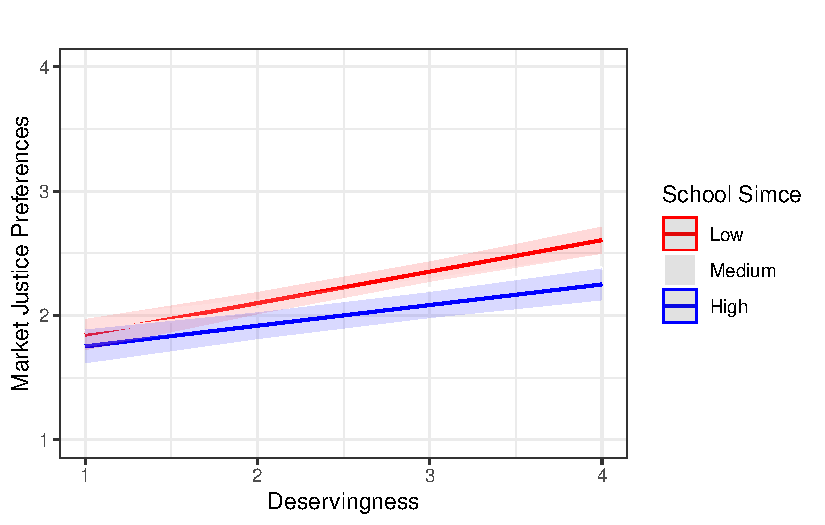
\includegraphics{paper_files/figure-pdf/fig-interaction-1.pdf}

}

\caption{\label{fig-interaction}Interaction between deservingness and
justification of inequality by school SIMCE achievement}

\end{figure}

\hypertarget{conclusion}{%
\subsection{Conclusion}\label{conclusion}}

\begin{itemize}
\tightlist
\item
  Efecto ilustrador de la educación? (esfuerzo -\textgreater{}
  redistribución)
\end{itemize}

\hypertarget{appendix}{%
\subsection{Appendix}\label{appendix}}

\begin{longtable}[]{@{}
  >{\raggedright\arraybackslash}p{(\columnwidth - 2\tabcolsep) * \real{0.4496}}
  >{\raggedright\arraybackslash}p{(\columnwidth - 2\tabcolsep) * \real{0.5504}}@{}}
\toprule()
\endhead
\textbf{English translation} & \textbf{Original Spanish} \\
It is just that in Chile people who cna pay have a better education for
their children & Es justo que en Chile las personas que puedan pagar
tengan una mejor educación para sus hijos. \\
It is just that in Chile people with higher incomes can have better
pensions than people with low incomes & Es justo que en Chile las
personas con mayores ingresos puedan tener mejores pensiones que las
personas de ingresos más bajos \\
It is just that in Chile people with higher incomes can access better
health services than people with low incomes & Es justo que en Chile las
personas con mayores ingresos puedan acceder a una mejor atención de
salud que las personas con ingresos más bajos \\
\bottomrule()
\end{longtable}

\hypertarget{refs}{}
\begin{CSLReferences}{1}{0}
\leavevmode\vadjust pre{\hypertarget{ref-acemoglu_obedience_2021}{}}%
Acemoglu, D. (2021). \emph{Obedience in the {Labor Market} and {Social
Mobility}: {A Socio-Economic Approach}} (No. w29125) (p. w29125).
Cambridge, MA: National Bureau of Economic Research.
\url{https://doi.org/10.3386/w29125}

\leavevmode\vadjust pre{\hypertarget{ref-almas_fairness_2017}{}}%
Almås, I., Cappelen, A. W., Salvanes, K. G., Sørensen, E. Ø., \&
Tungodden, B. (2017). Fairness and family background. \emph{Politics,
Philosophy \& Economics}, \emph{16}(2), 117--131.
\url{https://doi.org/10.1177/1470594X15618966}

\leavevmode\vadjust pre{\hypertarget{ref-almas_fairness_2010}{}}%
Almås, I., Cappelen, A. W., Sørensen, E. Ø., \& Tungodden, B. (2010).
Fairness and the {Development} of {Inequality Acceptance}.
\emph{Science}, \emph{328}(5982), 1176--1178.
\url{https://doi.org/10.1126/science.1187300}

\leavevmode\vadjust pre{\hypertarget{ref-almas_cutthroat_2020}{}}%
Almås, I., Cappelen, A. W., \& Tungodden, B. (2020). Cutthroat
{Capitalism} versus {Cuddly Socialism}: {Are Americans More
Meritocratic} and {Efficiency-Seeking} than {Scandinavians}?
\emph{Journal of Political Economy}, \emph{128}(5), 1753--1788.
\url{https://doi.org/10.1086/705551}

\leavevmode\vadjust pre{\hypertarget{ref-barr_effect_2020}{}}%
Barr, A., \& Miller, L. (2020). The effect of education, income
inequality and merit on inequality acceptance. \emph{Journal of Economic
Psychology}, \emph{80}, 102276.
\url{https://doi.org/10.1016/j.joep.2020.102276}

\leavevmode\vadjust pre{\hypertarget{ref-batruch_belief_2022}{}}%
Batruch, A., Jetten, J., Van de Werfhorst, H., Darnon, C., \& Butera, F.
(2022). Belief in {School Meritocracy} and the {Legitimization} of
{Social} and {Income Inequality}. \emph{Social Psychological and
Personality Science}, 194855062211110.
\url{https://doi.org/10.1177/19485506221111017}

\leavevmode\vadjust pre{\hypertarget{ref-bell_fixed_2019}{}}%
Bell, A., Fairbrother, M., \& Jones, K. (2019). Fixed and random effects
models: Making an informed choice. \emph{Quality \& Quantity},
\emph{53}(2), 1051--1074.
\url{https://doi.org/10.1007/s11135-018-0802-x}

\leavevmode\vadjust pre{\hypertarget{ref-boltanski_new_2005}{}}%
Boltanski, L., \& Chiapello, E. (2005). \emph{The new spirit of
capitalism}. London ; New York: Verso.

\leavevmode\vadjust pre{\hypertarget{ref-bourdieu_reproduction_1990}{}}%
Bourdieu, P., \& Passeron, J. C. (1990). \emph{Reproduction in
{Education}, {Society} and {Culture}} (Second Edition). Sage
Publications Ltd.

\leavevmode\vadjust pre{\hypertarget{ref-bucca_merit_2016}{}}%
Bucca, M. (2016). Merit and blame in unequal societies: {Explaining
Latin Americans}' beliefs about wealth and poverty. \emph{Research in
Social Stratification and Mobility}, \emph{44}, 98--112.
\url{https://doi.org/10.1016/j.rssm.2016.02.005}

\leavevmode\vadjust pre{\hypertarget{ref-castillo_legitimacy_2011}{}}%
Castillo, J. C. (2011). Legitimacy of {Inequality} in a {Highly Unequal
Context}: {Evidence} from the {Chilean Case}. \emph{Social Justice
Research}, \emph{24}(4), 314--340.
\url{https://doi.org/10.1007/s11211-011-0144-5}

\leavevmode\vadjust pre{\hypertarget{ref-castillo_meritocracia_2019}{}}%
Castillo, J. C., Torres, A., Atria, J., \& Maldonado, L. (2019).
Meritocracia y desigualdad econ{ó}mica: {Percepciones}, preferencias e
implicancias. \emph{Revista Internacional de Sociolog{í}a},
\emph{77}(1), 117. \url{https://doi.org/10.3989/ris.2019.77.1.17.114}

\leavevmode\vadjust pre{\hypertarget{ref-centeno_arc_2012}{}}%
Centeno, M. A., \& Cohen, J. N. (2012). The {Arc} of {Neoliberalism}.
\emph{Annual Review of Sociology}, \emph{38}(1), 317--340.
\url{https://doi.org/10.1146/annurev-soc-081309-150235}

\leavevmode\vadjust pre{\hypertarget{ref-chafel_schooling_1997}{}}%
Chafel, J. A. (1997). Schooling, the {Hidden Curriculum}, and
{Children}'s {Conceptions} of {Poverty}. \emph{Social Policy Report},
\emph{11}(1), 1--28.
\url{https://doi.org/10.1002/j.2379-3988.1997.tb00004.x}

\leavevmode\vadjust pre{\hypertarget{ref-chong_mystery_2008}{}}%
Chong, A., \& Ñopo, H. (2008). The {Mystery} of {Discrimination} in
{Latin America}. \emph{Econom{í}a}, \emph{8}(2), 79--107.
\url{https://doi.org/10.1353/eco.0.0005}

\leavevmode\vadjust pre{\hypertarget{ref-choudhury_social_2006}{}}%
Choudhury, S., Blakemore, S.-J., \& Charman, T. (2006). Social cognitive
development during adolescence. \emph{Social Cognitive and Affective
Neuroscience}, \emph{1}(3), 165--174.
\url{https://doi.org/10.1093/scan/nsl024}

\leavevmode\vadjust pre{\hypertarget{ref-darnon_where_2018}{}}%
Darnon, C., Wiederkehr, V., Dompnier, B., \& Martinot, D. (2018).
{``{Where} there is a will, there is a way''}: {Belief} in school
meritocracy and the social-class achievement gap. \emph{British Journal
of Social Psychology}, \emph{57}(1), 250--262.
\url{https://doi.org/10.1111/bjso.12214}

\leavevmode\vadjust pre{\hypertarget{ref-durante_preferences_2009}{}}%
Durante, R., \& Putterman, L. G. (2009). Preferences for
{Redistribution} and {Perception} of {Fairness}: {An Experimental
Study}. \emph{SSRN Electronic Journal}.
\url{https://doi.org/10.2139/ssrn.1004573}

\leavevmode\vadjust pre{\hypertarget{ref-duru-bellat_who_2012}{}}%
Duru-Bellat, M., \& Tenret, E. (2012). Who's for {Meritocracy}?
{Individual} and {Contextual Variations} in the {Faith}.
\emph{Comparative Education Review}, \emph{56}(2), 223--247.
\url{https://doi.org/10.1086/661290}

\leavevmode\vadjust pre{\hypertarget{ref-elenbaas_unfairness_2019}{}}%
Elenbaas, L. (2019). Against unfairness: {Young} children's judgments
about merit, equity, and equality. \emph{Journal of Experimental Child
Psychology}, \emph{186}, 73--82.
\url{https://doi.org/10.1016/j.jecp.2019.05.009}

\leavevmode\vadjust pre{\hypertarget{ref-engelmann_children_2019}{}}%
Engelmann, J. M., \& Tomasello, M. (2019). Children's {Sense} of
{Fairness} as {Equal Respect}. \emph{Trends in Cognitive Sciences},
\emph{23}(6), 454--463. \url{https://doi.org/10.1016/j.tics.2019.03.001}

\leavevmode\vadjust pre{\hypertarget{ref-erivwo_meritocracy_2021}{}}%
Erivwo, A., Varghese, E., Mathai, A., \& Afrin, T. (2021). Meritocracy
in the {Educational System}.
\url{https://doi.org/10.5281/ZENODO.4740695}

\leavevmode\vadjust pre{\hypertarget{ref-evans_strong_2018}{}}%
Evans, M. D. R., \& Kelley, J. (2018). Strong {Welfare States Do Not
Intensify Public Support} for {Income Redistribution}, but {Even Reduce
It} among the {Prosperous}: {A Multilevel Analysis} of {Public Opinion}
in 30 {Countries}. \emph{Societies}, \emph{8}(4), 105.
\url{https://doi.org/10.3390/soc8040105}

\leavevmode\vadjust pre{\hypertarget{ref-fernandez_positive_2013}{}}%
Fernandez, J. J., \& Jaime-Castillo, A. M. (2013). Positive or {Negative
Policy Feedbacks}? {Explaining Popular Attitudes Towards Pragmatic
Pension Policy Reforms}. \emph{European Sociological Review},
\emph{29}(4), 803--815. \url{https://doi.org/10.1093/esr/jcs059}

\leavevmode\vadjust pre{\hypertarget{ref-frank_performance_2015}{}}%
Frank, D. H., Wertenbroch, K., \& Maddux, W. W. (2015). Performance pay
or redistribution? {Cultural} differences in just-world beliefs and
preferences for wage inequality. \emph{Organizational Behavior and Human
Decision Processes}, \emph{130}, 160--170.
\url{https://doi.org/10.1016/j.obhdp.2015.04.001}

\leavevmode\vadjust pre{\hypertarget{ref-garcia-sanchez_attitudes_2020}{}}%
García-Sánchez, E., Osborne, D., Willis, G. B., \& Rodríguez-Bailón, R.
(2020). Attitudes towards redistribution and the interplay between
perceptions and beliefs about inequality. \emph{British Journal of
Social Psychology}, \emph{59}(1), 111--136.
\url{https://doi.org/10.1111/bjso.12326}

\leavevmode\vadjust pre{\hypertarget{ref-goldthorpe_myth_2003}{}}%
Goldthorpe, J. (2003). The myth of education-based meritocracy.
\emph{New Economy}, \emph{10}(4), 234--239.
\url{https://doi.org/10.1046/j.1468-0041.2003.00324.x}

\leavevmode\vadjust pre{\hypertarget{ref-goudeau_hidden_2017}{}}%
Goudeau, S., \& Croizet, J.-C. (2017). Hidden {Advantages} and
{Disadvantages} of {Social Class}: {How Classroom Settings Reproduce
Social Inequality} by {Staging Unfair Comparison}. \emph{Psychological
Science}, \emph{28}(2), 162--170.
\url{https://doi.org/10.1177/0956797616676600}

\leavevmode\vadjust pre{\hypertarget{ref-greitemeyer_subjective_2016}{}}%
Greitemeyer, T., \& Sagioglou, C. (2016). Subjective socioeconomic
status causes aggression: {A} test of the theory of social deprivation.
\emph{Journal of Personality and Social Psychology}, \emph{111}(2),
178--194. \url{https://doi.org/10.1037/pspi0000058}

\leavevmode\vadjust pre{\hypertarget{ref-harvey_breve_2015}{}}%
Harvey, D. (2015). \emph{{Breve historia del neoliberalismo}}. Madrid
(Espa{ñ}a): Ediciones Akal.

\leavevmode\vadjust pre{\hypertarget{ref-homan_being_2017}{}}%
Homan, P., Valentino, L., \& Weed, E. (2017). Being and {Becoming Poor}:
{How Cultural Schemas Shape Beliefs About Poverty}. \emph{Social
Forces}, \emph{95}(3), 1023--1048.
\url{https://doi.org/10.1093/sf/sox007}

\leavevmode\vadjust pre{\hypertarget{ref-hox_multilevel_2010}{}}%
Hox, J., Moerbeek, M., \& Schoot, R. van de. (2010). \emph{Multilevel
{Analysis}: {Techniques} and {Applications}, {Second Edition}} (2nd
ed.). New York: Routledge. \url{https://doi.org/10.4324/9780203852279}

\leavevmode\vadjust pre{\hypertarget{ref-huppert_development_2019}{}}%
Huppert, E., Cowell, J. M., Cheng, Y., Contreras-Ibáñez, C.,
Gomez-Sicard, N., Gonzalez-Gadea, M. L., \ldots{} Decety, J. (2019). The
development of children's preferences for equality and equity across 13
individualistic and collectivist cultures. \emph{Developmental Science},
\emph{22}(2), e12729. \url{https://doi.org/10.1111/desc.12729}

\leavevmode\vadjust pre{\hypertarget{ref-hvidberg_social_2023}{}}%
Hvidberg, K. B., Kreiner, C. T., \& Stantcheva, S. (2023). Social
{Positions} and {Fairness Views} on {Inequality}. \emph{Review of
Economic Studies}, \emph{90}(6), 3083--3118.
\url{https://doi.org/10.1093/restud/rdad019}

\leavevmode\vadjust pre{\hypertarget{ref-iacoviello_collectivism_2019}{}}%
Iacoviello, V., \& Lorenzi-Cioldi, F. (2019). Collectivism and
{Individualism} in {Status Hierarchies}: {Socialization} and {Social
Identity Explanations}. \emph{International Review of Social
Psychology}, \emph{32}(1), 15. \url{https://doi.org/10.5334/irsp.285}

\leavevmode\vadjust pre{\hypertarget{ref-jack_no_2016}{}}%
Jack, A. A. (2016). ({No}) {Harm} in {Asking}: {Class}, {Acquired
Cultural Capital}, and {Academic Engagement} at an {Elite University}.
\emph{Sociology of Education}, \emph{89}(1), 1--19.
\url{https://doi.org/10.1177/0038040715614913}

\leavevmode\vadjust pre{\hypertarget{ref-jasso_how_1999}{}}%
Jasso, G. (1999). How {Much Injustice} is {There} in the {World}? {Two
New Justice Indexes}. \emph{American Sociological Review}, \emph{64}(1),
133--168. \url{https://doi.org/10.1177/000312249906400110}

\leavevmode\vadjust pre{\hypertarget{ref-jensen_worlds_2008}{}}%
Jensen, C. (2008). Worlds of welfare services and transfers.
\emph{Journal of European Social Policy}, \emph{18}(2), 151--162.
\url{https://doi.org/10.1177/0958928707087591}

\leavevmode\vadjust pre{\hypertarget{ref-jonsson_institutional_2015}{}}%
Jonsson, A.-C., \& Beach, D. (2015). Institutional discrimination:
{Stereotypes} and social reproduction of {``class''} in the {Swedish}
upper-secondary school. \emph{Social Psychology of Education},
\emph{18}(4), 703--717. \url{https://doi.org/10.1007/s11218-014-9279-1}

\leavevmode\vadjust pre{\hypertarget{ref-jost_attitudinal_2000}{}}%
Jost, J. T., \& Burgess, D. (2000). Attitudinal {Ambivalence} and the
{Conflict} between {Group} and {System Justification Motives} in {Low
Status Groups}. \emph{Personality and Social Psychology Bulletin},
\emph{26}(3), 293--305. \url{https://doi.org/10.1177/0146167200265003}

\leavevmode\vadjust pre{\hypertarget{ref-khan_privilege_2011}{}}%
Khan, S. (2011). \emph{Privilege: {The Making} of an {Adolescent Elite}
at {St}. {Paul}'s {School}}. Princeton, N.J.: Princeton University
Press.

\leavevmode\vadjust pre{\hypertarget{ref-kluegel_beliefs_1987}{}}%
Kluegel, J. R., \& Smith, E. R. (1987). \emph{Beliefs about inequality:
{Americans}' views of what is and what ought to be}. London New York:
Routledge, Taylor \& Francis Group.

\leavevmode\vadjust pre{\hypertarget{ref-kohn_social_1963}{}}%
Kohn, M. L. (1963). Social {Class} and {Parent-Child Relationships}: {An
Interpretation}. \emph{American Journal of Sociology}, \emph{68}(4),
471--480. \url{https://doi.org/10.1086/223403}

\leavevmode\vadjust pre{\hypertarget{ref-kohn_class_1969}{}}%
Kohn, M. L., \& Schooler, C. (1969). Class, {Occupation}, and
{Orientation}. \emph{American Sociological Review}, \emph{34}(5), 659.
\url{https://doi.org/10.2307/2092303}

\leavevmode\vadjust pre{\hypertarget{ref-kosse_prosociality_2020}{}}%
Kosse, F., \& Tincani, M. M. (2020). Prosociality predicts labor market
success around the world. \emph{Nature Communications}, \emph{11}(1),
5298. \url{https://doi.org/10.1038/s41467-020-19007-1}

\leavevmode\vadjust pre{\hypertarget{ref-lampert_meritocratic_2013}{}}%
Lampert, K. (2013). \emph{Meritocratic {Education} and {Social
Worthlessness}}. London: Palgrave Macmillan UK.
\url{https://doi.org/10.1057/9781137324894}

\leavevmode\vadjust pre{\hypertarget{ref-lane_market_1986}{}}%
Lane, R. E. (1986). Market {Justice}, {Political Justice}.
\emph{American Political Science Review}, \emph{80}(2), 383--402.
\url{https://doi.org/10.2307/1958264}

\leavevmode\vadjust pre{\hypertarget{ref-lindh_public_2015}{}}%
Lindh, A. (2015). Public {Opinion} against {Markets}? {Attitudes}
towards {Market Distribution} of {Social Services} -- {A Comparison} of
17 {Countries}. \emph{Social Policy \& Administration}, \emph{49}(7),
887--910. \url{https://doi.org/10.1111/spol.12105}

\leavevmode\vadjust pre{\hypertarget{ref-mcauliffe_developmental_2017}{}}%
McAuliffe, K., Blake, P. R., Steinbeis, N., \& Warneken, F. (2017). The
developmental foundations of human fairness. \emph{Nature Human
Behaviour}, \emph{1}(2), 0042.
\url{https://doi.org/10.1038/s41562-016-0042}

\leavevmode\vadjust pre{\hypertarget{ref-mijs_stratified_2016}{}}%
Mijs, J. (2016). Stratified {Failure}: {Educational Stratification} and
{Students}' {Attributions} of {Their Mathematics Performance} in 24
{Countries}. \emph{Sociology of Education}, \emph{89}(2), 137--153.
\url{https://doi.org/10.1177/0038040716636434}

\leavevmode\vadjust pre{\hypertarget{ref-mijs_paradox_2021}{}}%
Mijs, J. (2021). The paradox of inequality: Income inequality and belief
in meritocracy go hand in hand. \emph{Socio-Economic Review},
\emph{19}(1), 7--35. \url{https://doi.org/10.1093/ser/mwy051}

\leavevmode\vadjust pre{\hypertarget{ref-mikus_children_2020}{}}%
Mikus, K., Tieben, N., \& Schober, P. S. (2020). Children's conversion
of cultural capital into educational success: The symbolic and
skill-generating functions of cultural capital. \emph{British Journal of
Sociology of Education}, \emph{41}(2), 197--217.
\url{https://doi.org/10.1080/01425692.2019.1677454}

\leavevmode\vadjust pre{\hypertarget{ref-mishra_subjective_2015}{}}%
Mishra, S., \& Carleton, R. N. (2015). Subjective relative deprivation
is associated with poorer physical and mental health. \emph{Social
Science \& Medicine}, \emph{147}, 144--149.
\url{https://doi.org/10.1016/j.socscimed.2015.10.030}

\leavevmode\vadjust pre{\hypertarget{ref-molyneux_neoliberal_2008}{}}%
Molyneux, M. (2008). The {``{Neoliberal Turn}''} and the {New Social
Policy} in {Latin America}: {How Neoliberal}, {How New}?
\emph{Development and Change}, \emph{39}(5), 775--797.
\url{https://doi.org/10.1111/j.1467-7660.2008.00505.x}

\leavevmode\vadjust pre{\hypertarget{ref-morris_representing_2022}{}}%
Morris, J., Reilly, J., Paltsev, S., Sokolov, A., \& Cox, K. (2022).
Representing {Socio}-{Economic Uncertainty} in {Human System Models}.
\emph{Earth's Future}, \emph{10}(4), e2021EF002239.
\url{https://doi.org/10.1029/2021EF002239}

\leavevmode\vadjust pre{\hypertarget{ref-pierson_increasing_2000}{}}%
Pierson, P. (2000). Increasing {Returns}, {Path Dependence}, and the
{Study} of {Politics}. \emph{American Political Science Review},
\emph{94}(2), 251--267. \url{https://doi.org/10.2307/2586011}

\leavevmode\vadjust pre{\hypertarget{ref-power_deprivationprotest_2018}{}}%
Power, Séamus A. (2018). The {Deprivation-Protest Paradox}: {How} the
{Perception} of {Unfair Economic Inequality Leads} to {Civic Unrest}.
\emph{Current Anthropology}, \emph{59}(6), 765--789.
\url{https://doi.org/10.1086/700679}

\leavevmode\vadjust pre{\hypertarget{ref-power_relative_2020}{}}%
Power, Séamus A., Madsen, T., \& Morton, T. A. (2020). Relative
deprivation and revolt: Current and future directions. \emph{Current
Opinion in Psychology}, \emph{35}, 119--124.
\url{https://doi.org/10.1016/j.copsyc.2020.06.010}

\leavevmode\vadjust pre{\hypertarget{ref-resh_sense_2010}{}}%
Resh, N. (2010). Sense of justice about grades in school: Is it
stratified like academic achievement? \emph{Social Psychology of
Education}, \emph{13}(3), 313--329.
\url{https://doi.org/10.1007/s11218-010-9117-z}

\leavevmode\vadjust pre{\hypertarget{ref-resh_sense_2014}{}}%
Resh, N., \& Sabbagh, C. (2014). Sense of justice in school and civic
attitudes. \emph{Social Psychology of Education}, \emph{17}(1), 51--72.
\url{https://doi.org/10.1007/s11218-013-9240-8}

\leavevmode\vadjust pre{\hypertarget{ref-resh_sense_2017}{}}%
Resh, N., \& Sabbagh, C. (2017). Sense of justice in school and civic
behavior. \emph{Social Psychology of Education}, \emph{20}(2), 387--409.
\url{https://doi.org/10.1007/s11218-017-9375-0}

\leavevmode\vadjust pre{\hypertarget{ref-salamon_marketization_1993}{}}%
Salamon, L. M. (1993). The {Marketization} of {Welfare}: {Changing
Nonprofit} and {For-Profit Roles} in the {American Welfare State}.
\emph{Social Service Review}, \emph{67}(1), 16--39.
\url{https://doi.org/10.1086/603963}

\leavevmode\vadjust pre{\hypertarget{ref-salgado_inequality_2023}{}}%
Salgado, M., \& Castillo, J. (2023). Inequality and {Stratification} in
{Latin America}. In M. Gangl, L. Platt, J. G. Polavieja, \& H. G. van de
Werfhorst (Eds.), \emph{The {Oxford Handbook} of {Social
Stratification}} (p. 0). 2023: Oxford University Press.

\leavevmode\vadjust pre{\hypertarget{ref-sandel_tyranny_2020}{}}%
Sandel, M. J. (2020). \emph{The tyranny of merit: {What}'s become of the
common good?} (First edition). New York: {Farrar, Straus and Giroux}.

\leavevmode\vadjust pre{\hypertarget{ref-schunk_fairness_2023}{}}%
Schunk, D., \& Zipperle, I. (2023). Fairness and inequality acceptance
in children and adolescents: {A} survey on behaviors in economic
experiments, \emph{37}(5), 1715--1742.
\url{https://doi.org/10.1111/joes.12553}

\leavevmode\vadjust pre{\hypertarget{ref-shariff_income_2016}{}}%
Shariff, A. F., Wiwad, D., \& Aknin, L. B. (2016). Income {Mobility
Breeds Tolerance} for {Income Inequality}: {Cross-National} and
{Experimental Evidence}. \emph{Perspectives on Psychological Science},
\emph{11}(3), 373--380. \url{https://doi.org/10.1177/1745691616635596}

\leavevmode\vadjust pre{\hypertarget{ref-sigelman_development_1991}{}}%
Sigelman, C. K., \& Waitzman, K. A. (1991). The {Development} of
{Distributive Justice Orientations}: {Contextual Influences} on
{Children}'s {Resource Allocations}. \emph{Child Development},
\emph{62}(6), 1367. \url{https://doi.org/10.2307/1130812}

\leavevmode\vadjust pre{\hypertarget{ref-sivesind_changing_2017}{}}%
Sivesind, K. H. (2017). The {Changing Roles} of {For-Profit} and
{Nonprofit Welfare Provision} in {Norway}, {Sweden}, and {Denmark}. In
K. H. Sivesind \& J. Saglie (Eds.), \emph{Promoting {Active
Citizenship}} (pp. 33--74). Cham: Springer International Publishing.
\url{https://doi.org/10.1007/978-3-319-55381-8_2}

\leavevmode\vadjust pre{\hypertarget{ref-smith_relative_2012}{}}%
Smith, H. J., Pettigrew, T. F., Pippin, G. M., \& Bialosiewicz, S.
(2012). Relative {Deprivation}: {A Theoretical} and {Meta-Analytic
Review}. \emph{Personality and Social Psychology Review}, \emph{16}(3),
203--232. \url{https://doi.org/10.1177/1088868311430825}

\leavevmode\vadjust pre{\hypertarget{ref-soler-martinez_concerns_2023}{}}%
Soler-Martínez, F. M., García-Sánchez, E., \& Willis, G. B. (2023).
Concerns {About Inequality} in {Health}, {Education} and {Income Jointly
Predict Collective Actions}. \emph{Revista Latinoamericana de
Psicolog{í}a}, \emph{55}, 99.
\url{https://doi.org/10.14349/rlp.2023.v55.12}

\leavevmode\vadjust pre{\hypertarget{ref-stoy_worlds_2014}{}}%
Stoy, V. (2014). Worlds of {Welfare Services}: {From Discovery} to
{Exploration}. \emph{Social Policy \& Administration}, \emph{48}(3),
343--360. \url{https://doi.org/10.1111/spol.12006}

\leavevmode\vadjust pre{\hypertarget{ref-streeck_citizens_2012}{}}%
Streeck, W. (2012). Citizens as {Customers}: {Considerations} on the
{New Politics} of {Consumption}. \emph{New Left Review}, \emph{76}.

\leavevmode\vadjust pre{\hypertarget{ref-torche_intergenerational_2014}{}}%
Torche, F. (2014). Intergenerational {Mobility} and {Inequality}: {The
Latin American Case}. \emph{Annual Review of Sociology}, \emph{40}(1),
619--642. \url{https://doi.org/10.1146/annurev-soc-071811-145521}

\leavevmode\vadjust pre{\hypertarget{ref-vonhippel_test_2019}{}}%
Von Hippel, P., \& Hamrock, C. (2019). Do {Test Score Gaps Grow} before,
during, or between the {School Years}? {Measurement Artifacts} and {What
We Can Know} in {Spite} of {Them}. \emph{Sociological Science},
\emph{6}, 43--80. \url{https://doi.org/10.15195/v6.a3}

\leavevmode\vadjust pre{\hypertarget{ref-weaver_paths_2010}{}}%
Weaver, K. (2010). Paths and {Forks} or {Chutes} and {Ladders}?:
{Negative Feedbacks} and {Policy Regime Change}. \emph{Journal of Public
Policy}, \emph{30}(2), 137--162.
\url{https://doi.org/10.1017/S0143814X10000061}

\leavevmode\vadjust pre{\hypertarget{ref-wegener_dominant_1995}{}}%
Wegener, B., \& Liebig, S. (1995). Dominant {Ideologies} and the
{Variation} of {Distributive Justice Norms}: {A Comparison} of {East}
and {West Germany}, and the {United States}. In J. R. Kluegel, D. S.
Mason, \& B. Wegener (Eds.), \emph{Social {Justice} and {Political
Change}: {Public Opinion} in {Capitalist} and {Post-Communist States}}
(pp. 239--259). New York: Walter de Gruyter.

\leavevmode\vadjust pre{\hypertarget{ref-wiederkehr_belief_2015}{}}%
Wiederkehr, V., Bonnot, V., Krauth-Gruber, S., \& Darnon, C. (2015).
Belief in school meritocracy as a system-justifying tool for low status
students. \emph{Frontiers in Psychology}, \emph{6}.

\leavevmode\vadjust pre{\hypertarget{ref-wynn_not_2018}{}}%
Wynn, K., Bloom, P., Jordan, A., Marshall, J., \& Sheskin, M. (2018).
Not {Noble Savages After All}: {Limits} to {Early Altruism}.
\emph{Current Directions in Psychological Science}, \emph{27}(1), 3--8.
\url{https://doi.org/10.1177/0963721417734875}

\leavevmode\vadjust pre{\hypertarget{ref-young_rise_1958}{}}%
Young, M. (1958). \emph{The rise of the meritocracy}. New Brunswick,
N.J., U.S.A: Transaction Publishers.

\end{CSLReferences}



\end{document}
